\documentclass[12pt]{article}

\usepackage{graphicx}
\usepackage{amsmath}
\usepackage{amsfonts}
\usepackage[style=authoryear, natbib=true, url=false, isbn=false, doi=false, backend=bibtex]{biblatex}
\usepackage[margin=1in]{geometry}
\usepackage[doublespacing]{setspace}

\renewcommand*{\nameyeardelim}{\addcomma\addspace}
\bibliography{ZoteroLibrary}
\renewbibmacro{in:}{}

% arara: pdflatex 
% arara: bibtex 
% arara: pdflatex 
% arara: pdflatex 
\begin{document}

\title{Effective Data Science Education: \\
\large A Project-Based Case Study Perspective}

\author{Daniel Turek$^{*}$, Anthony Suen, Dav Clark}

\date{}

\maketitle

\vspace{0.4in}
\begin{center}

Berkeley Institute for Data Science \\
University of California \\
Berkeley, CA 94720, USA

\vspace{0.8in}

$^*$Corresponding Author \\
dturek@berkeley.edu
\end{center}

\thispagestyle{empty}
\newpage

\begin{abstract}
The discipline of data science has been viewed as a convergence of high-power computing, data visualization and analysis, and data-driven application domains over the past decade.  Prominent research institutions and private sector industry have embraced data science, but the foundations for effective tertiary-level data science education are conspicuously absent. This is nothing new, however, as the university has a well-established tradition of developing its educational mission hand-in-hand with the development of novel methods for human understanding \citep{feingold_tradition_1991}. Thus, it is natural that universities ``figure out" data science concurrent with the development of needed pedagogy. We consider the development of data science education with respect to recent trends in interdisciplinary and experiential methodologies to understand how they could apply to data science education programs. These perspectives motivate us to consider what factors are necessary to drive effective data science education, which range from a complete end-to-end workflow, technological tools for development and team communications, and appropriate motivation and incentives. The first iteration of the \emph{Berkeley Institute for Data Science (BIDS) Collaborative} started in the University of California, Berkeley in the Spring of 2015 is used as a case study. From this, we draw lessons learned and form a hypothesis regarding the necessary ingredients for effective data science education at the tertiary level -- a topic that is presently understudied.  This hypothesis will be tested and revised in subsequent iterations of the BIDS Collaborative as we continue our study of data science education, research, and social impact.
\end{abstract}

\vspace{0.4in}

\textbf{Keywords:} \\
\indent \indent Data science, Tertiary education, Case study, Experiential learning

\thispagestyle{empty}
\newpage

\section{Introduction}

Owing to the rapid advances in computational power and the on-going ``big data" craze, the discipline of data science has exploded onto the academic and business landscape. Master's programs in data science are now being offered at leading research institutions such as Stanford University and Columbia University, and centers for data science have recently opened their doors at the University of California, Berkeley, the University of Washington, and New York University. Led  by the success of tech giants such as Google, Amazon and Facebook, the increasing availability of data is transforming industries ranging from medicine to media.  The industrial sector is keeping pace by creating and actively recruiting for positions in data science.  The profession of data scientist was even described by the Harvard Business Review as ``the sexiest job of the 21$^{\text{st}}$ century" \citep{Patil2012}.

Despite this inundation of the term ``data science," we still struggle to define what data science is, or to realize any boundaries as to what data science encompasses \citep{Hayashi1998, Loukides2011, Provost2013}. A common Venn diagram places data science squarely at the intersection of computer science, mathematical statistics, and scientific application domains.  This perhaps most accurately depicts that data science is nebulous by nature, having ties to all areas of quantitative scientific research or computational data analysis, but falls short of providing an understanding of how this new scientific discipline will eventually settle into the scientific ecosystem.  Fortunately, our aim is not to pin down the nature of data science itself, but instead to examine the practicalities and realities of data science education at the tertiary level.

There exists substantial literature regarding best practices and modern approaches to tertiary education. This has been a subject of interest since the first modern Universities appeared in Europe \citep{Rudy1984, Pedersen1997}.  Since then, the approach to higher education has evolved immensely, due to advances in technology, and also society's attitude towards higher education.  Perhaps the single-most transformative influence on higher education has been the so-called digital revolution of the past decades, which has had a profound impact on the content and style of tertiary education \citep{Roberts1994, Ely1995, Baker1997, Wood2005, Baek2008}.

Some research suggests that traditional approaches to tertiary education may only result in superficial learning, rather than a deep understanding of subject material \citep{Entwistle1992}.  Thus, the study of education itself is an area of prime interest.  Many approaches have been suggested and studied over the past decades, in attempts to improve tertiary education.  \citet{Topping1996} promotes the practice of peer-tutoring, while others have more recently endorsed ``flipped classrooms" in which learning is more self-directed rather than instructor-directed, and classrooms become a place for practice instead of lecture \citep{Horn2013, Herreid2013}.  \citet{Ogawa1995} suggests a ``mutiscience" approach to multidisciplinary science education, in which the diversity scientific disciplines is recognized and incorporated into the educational system.  The approach of constructive alignment is an example of outcome-based education, in which teaching and assessments are constructed to naturally align with the desired educational outcomes \citep{biggs2003aligning, biggs2011teaching}.  Project-based learning has been promoted at the institutional level for many years \citep{Krajcik2006, Thomas2000}.

The focus of our analysis is specifically the education of data science. In light of the academic and industry spotlight on data science, experiences and best practices for data science education should be an active area of research, just as it is for tertiary education in general.  However, owing to its relatively recent mainstream debut, there is an absence of scientific research or published literature on data science education.  This fact motivates our present analysis of the history, current trends, and future prospects of data science education.

We aim to begin filling this void by providing a tangible case study of data science education, which was undertaken at the University of California, Berkeley, under the BIDS Collaborative. We consider the successes and failures of the first cohort to pass through the BIDS Collaborative, and the pain points which were encountered by the students and mentors, alike.  We make practical recommendations for educational approaches to data science curricula, and formulate a hypothesis regarding the ``best practices" of tertiary data science education.  Study of our hypothesis will require subsequent experiential testing, which will be the subject of on-going and future research.



\section{Paradigms of Science Education}

To set the context for data science training and research methods, we briefly review several educational paradigms that have become prominent in the past few decades. These include interdisciplinary research and the experiential learning educational model. We also consider the Data Science for Social Good model (DSSG; \texttt{http://dssg.io}), which has been used in Chicago for training approximately 50 graduate students in data science each summer since 2013. Finally, we will break down from these paradigms the theories we hope to practice in the BIDS Collaborative.

\subsection{Interdisciplinary Research}

Interdisciplinary or multidisciplinary research is ``a format for conversation and connections that will lead to new knowledge" \citep{repko2008interdisciplinary}. The word has been a fashionable academic buzzword for decades now, but the approach of looking at and solving issues from multiple angles has failed to fundamentally scale beyond the confines of certain research groups to change the way research is carried out. There are major obstacles like cultural, organizational, technical barriers that prevent such learning and research environments \citep{eisenberg2000bridging}.

First, interdisciplinary training is not generally taught, whether you are an undergraduate or graduate student. Interdisciplinary is not a core metric for industry or academic career paths in order to be exposed to the values. This lack of training is due in part to organizational structure with many departments providing little to no incentives for interdisciplinary collaborations. By making job prospects for those who have multidisciplinary focus difficult, it creates a self-propagating cycle that reinforces single disciplinary specialist work. 

These organizational structures also created silos around sets of tools -- different software and methods are used to achieve similar goals via widely divergent means, potentially obscuring the fact that disparate groups are in fact grappling with the same underlying problems. Social scientists, physical sciences, and engineering use very different tools to tackle data. They use these different tools to run models that often have similar predictive goals. For example, Stata \citep{stata2005stata} might be used by an economist, Matlab \citep{incorporation2005matlab} by the engineer, and R \citep{RCoreTeam2014} by the statistician. This divergence and specialization in tools creates an ever widening gap between major disciplines.  These pose obstacles to true interdisciplinary collaboration among diverse teams of researchers.

Observing these barriers to multidisciplinary data science, our mission was three-fold. First, we implemented a framework for interdisciplinary learning beyond traditional academic lecture and coursework structures. Second, we cultivated an environment independent of the ``rules" or established incentive structure of traditional academic departments. Our third goal was to show interdisciplinarity was possible with limited resources and incentives, and that data science tools can be readily shared across disciplines. 

This mission highlights a need for leaders within multidisciplinary teams which might be easier to achieve in a graduate student and undergraduate student teams than among faculty due to lower barriers in terms of technology, incentives, and generally a stronger feeling of openness to approaching problems in a new way. We hypothesized that multidisciplinary collaboration would be easier when the stakes are smaller than traditional academics and learning is driven within student peer groups.

\subsection{Experiential Learning (Flipped Classroom)}

We supported our interdisciplinary mission with projects that were genuinely experientially focused.  This involved external clients and real-world data. Under this model, students no longer played passive roles in the educational process, but instead their active participation drove the educational mechanism \citep{beard2010experiential}. Instead of teachers ``transmitting" knowledge, mentors and facilitators ensured that projects and learning were on track, and that needed resources were available. This model for education is also known as a ``flipped classroom."

Research from Stanford University \citep{plotnikoff_classes_2013} has validated that the flipped class experiential learning is a stronger learning strategy compared to the traditional approach of combining lectures and homework. Students being required to actively contribute, without advance lecture preparation has been shown to be effective in accelerating knowledge acquisition. This experiential approach means removing the accepted format of lectures and tests entirely. 

Experiential learning also emphasizes project management, since classroom projects have clear deadlines scheduled imposed by the professor \citep{mok2014teaching}. Given the diverse nature of each project, our limited staffing resources, and the need to manage relationships with clients, it was critical that students -- the team leads, in particular -- naturally assumed roles as project managers.  The provided the guidance and motivation for teams to push forward throughout the semester, without continuous intervention from facilitators. As an added benefit, the experiential learning approach is also a more realistic representation of practical data science outside the classroom.



\section{Case Study: BIDS Collaborative}

The central organizing principle of the collaborative was to organize teams of students around data science projects. In data science education, project domains and materials must be relevant to student backgrounds. Thus, one of our primary concerns was to ensure projects that would be of interest to a wide variety of students, and we therefore collected a diverse set of 16 projects. 

Based on lessons learned from the DSSG program, we requested that project clients have data ready in hand that they were able to share with student teams. We also attempted to ensure that projects were clearly framed as an answerable question. It seems clear in hindsight, however, that student enthusiasm for a project was driven almost entirely by the presence of the ``client" to give a pitch to students during one of two informational sessions at the beginning of the semester. Given limited time and resources for managing the Collaborative, most client proposals were not vetted for data availability. Four projects received sufficient student interest for team formation and undertaking successful research.

We first describe the projects which made up the first iteration of the BIDS Collaborative.  Next we detail of the process of project selection and team formation which ultimately resulted in these projects.  We also provide an analysis of the tools used and temporal workflows compared among project teams, relating these to the successes and challenges experienced by each team.

\subsection{Projects}

The first iteration of the BIDS Collaborative consisted of four data science research projects.

\subsubsection*{DeStress: Text Mining for Stress}

This was one of two projects that was driven by faculty involvement. What differentiated these projects from standard faculty-driven research was the inclusive call for participation, and the engagement in a collaborative open-source development framework. This project pursued Berkeley Professor of Computer Science John Canny's BIDMach system (\texttt{http://bid2.berkeley.edu/bid-data-project/}; \cite{canny2013bidmach}) -- a performant GPU-accelerated system for machine learning in the Scala language. A domain focus on determining stress and major life events using large-scale machine learning was chosen by one of Professor Canny's graduate students, Pablo Paredes.

The project was enabled in part by providing a commodity workstation that was already available in the D-Lab, with the addition 1TB of hard disk storage. Thus, while this project was pushing the limits of academic machine learning, the resources for this project would be readily accessible to modestly funded labs.  The DeStress project and code is available at \texttt{https://github.com/berkeley-dsc/destress}.

\subsubsection*{Underclub: Online Business Feedback Analysis}

While our intention was to primarily recruit clients from outside the university, Underclub was the only client that approximated this intent. Indeed, even they had a pre-existing affiliation with the university via the Haas school of business.  In this project, students analyzed survey response data from a start-up company centered around online clothing distribution and sales.  Using this data, recommendations were made for the business client regarding how to appropriately address market segmentation and the inherent challenges of online marketplaces.  Given the business-related nature of this work, it was carried out in a private repository.

\subsubsection*{Finance: Analyzing Financial Market Data with Apache Spark}

This project was the second of two that was driven by a faculty member, in this case, Berkeley Professor Justin McCrary, faculty director of the D-Lab. Professor McCrary has been working to develop efficient workflows to take advantage of the UC Berkeley campus compute cluster, Savio. To this end, we worked with the Berkeley Research Computing team that manages the cluster to enable a modern Spark-based workflow (\texttt{http://spark.apache.org/}).

This project was likely of the highest value to campus, as it improved the ability to take advantage of the impressive parallel capabilities that are now provided to all senior campus researchers as a ``birthright" -- particularly for those users who may need something other than a traditional HPC workflow. This code was maintained and organized at \texttt{https://github.com/berkeley-dsc/dlab-finance}.

\subsubsection*{Purchasing: University of California Berkeley Strategic Sourcing}

The director of the University of California's strategic sourcing unit had a pre-existing connection with the Berkeley D-Lab (\texttt{http://dlab.berkeley.edu/}) via a previous analyst's use of D-Lab python training and consulting. This work led to a conference talk at SciPy 2014 discussing how straightforward scientific python scripts were able to accelerate previously spreadsheet-based analyses from taking approximately a week to a matter of minutes. A Collaborative facilitator assisted strategic sourcing in this work, and was therefore aware of the opportunities available to save the university system time and money. From the perspective of an academic institution, this project illustrates an exciting double-win, with potential benefits both to Berkeley administration and student training.  The project was organized at \texttt{https://github.com/berkeley-dsc/purchasing}.

\subsection{Project Selection and Team Formation}

The BIDS Collaborative ran four projects during the course of the semester, with clients from industry, academia, non-profit, and government. Each project followed a somewhat idiosyncratic course, though there were clear commonalities, both in terms of challenges and solutions. Teams consisted of between four and six members drawn from various academic disciplines. A particular concern was the need to balance the technical skills and experience present in each team.

Team formation was somewhat chaotic and arguably the most difficult part of the process from the facilitator perspective. Participants were largely attracted via two ``mixers" at the beginning of the Spring 2015 semester, which consisted of a brief motivational presentation after which students were encouraged to discuss their research interests, and form teams around one of the available projects. Students were given a large number of choices, and were encouraged to organize themselves via an online spreadsheet. While self-organization might work more efficiently via a system that could enforce a set of rules and policies, allowing all students to collaboratively edit a spreadsheet created numerous problems. The most dramatic difficulty occurred when a large number of student responses were inadvertently deleted from the spreadsheet.

Ultimately, our efforts to create a ``self-service" approach required facilitators in the Collaborative to engage in a very time-intensive process, organizing teams via extensive conversations in person and via email. While attendance at the mixers was quite strong, the Collaborative ultimately retained thirteen individuals from the initial cohort, with an additional three joining several weeks into the semester. One individual dropped off mid-semester, though participation was otherwise stable thereafter.

An additional challenge at the beginning of the Spring 2015 semester was the lack of leadership in the various teams. Teams could best be described as loose assemblies of individuals working relatively independently on related topics, and progress was slow. Recognizing this lack of cohesion, we suggested that each team choose a lead -- a process that generally consisted of one person volunteering to take on this role. At least one individual expressed reluctance to engage in a management role, as their interest was largely in hands-on experience. Moreover, after this transition, it was often difficult for these reluctant managers to lead their teams.  At this stage, team leads served a gatekeeper function in allowing students into their team. For these students, the authority of the team lead appeared to be more established. To be clear, ``authority" here was very gently exercised, and primarily consisted of working with facilitators to be clear about intended work, and progress achieved.

\subsection{Tools and Workflows}

While both the facilitators and participating teams were divided on the issue at first, all teams switched to development on GitHub early in the semester. Teams formed in mid-February, and all teams were committing to GitHub by March, consistent with training sessions in using these collaborative tools.  The GitHub usage commit history of each team is shown in Figure~\ref{fig:gitcommits}, the data for which is publicly available at individual project websites.  These GitHub commit histories are presented alongside the project management workflow employed by the Collaborative facilitators, and the research workflows that project teams were encouraged to follow.

\begin{figure*}
%\centerline{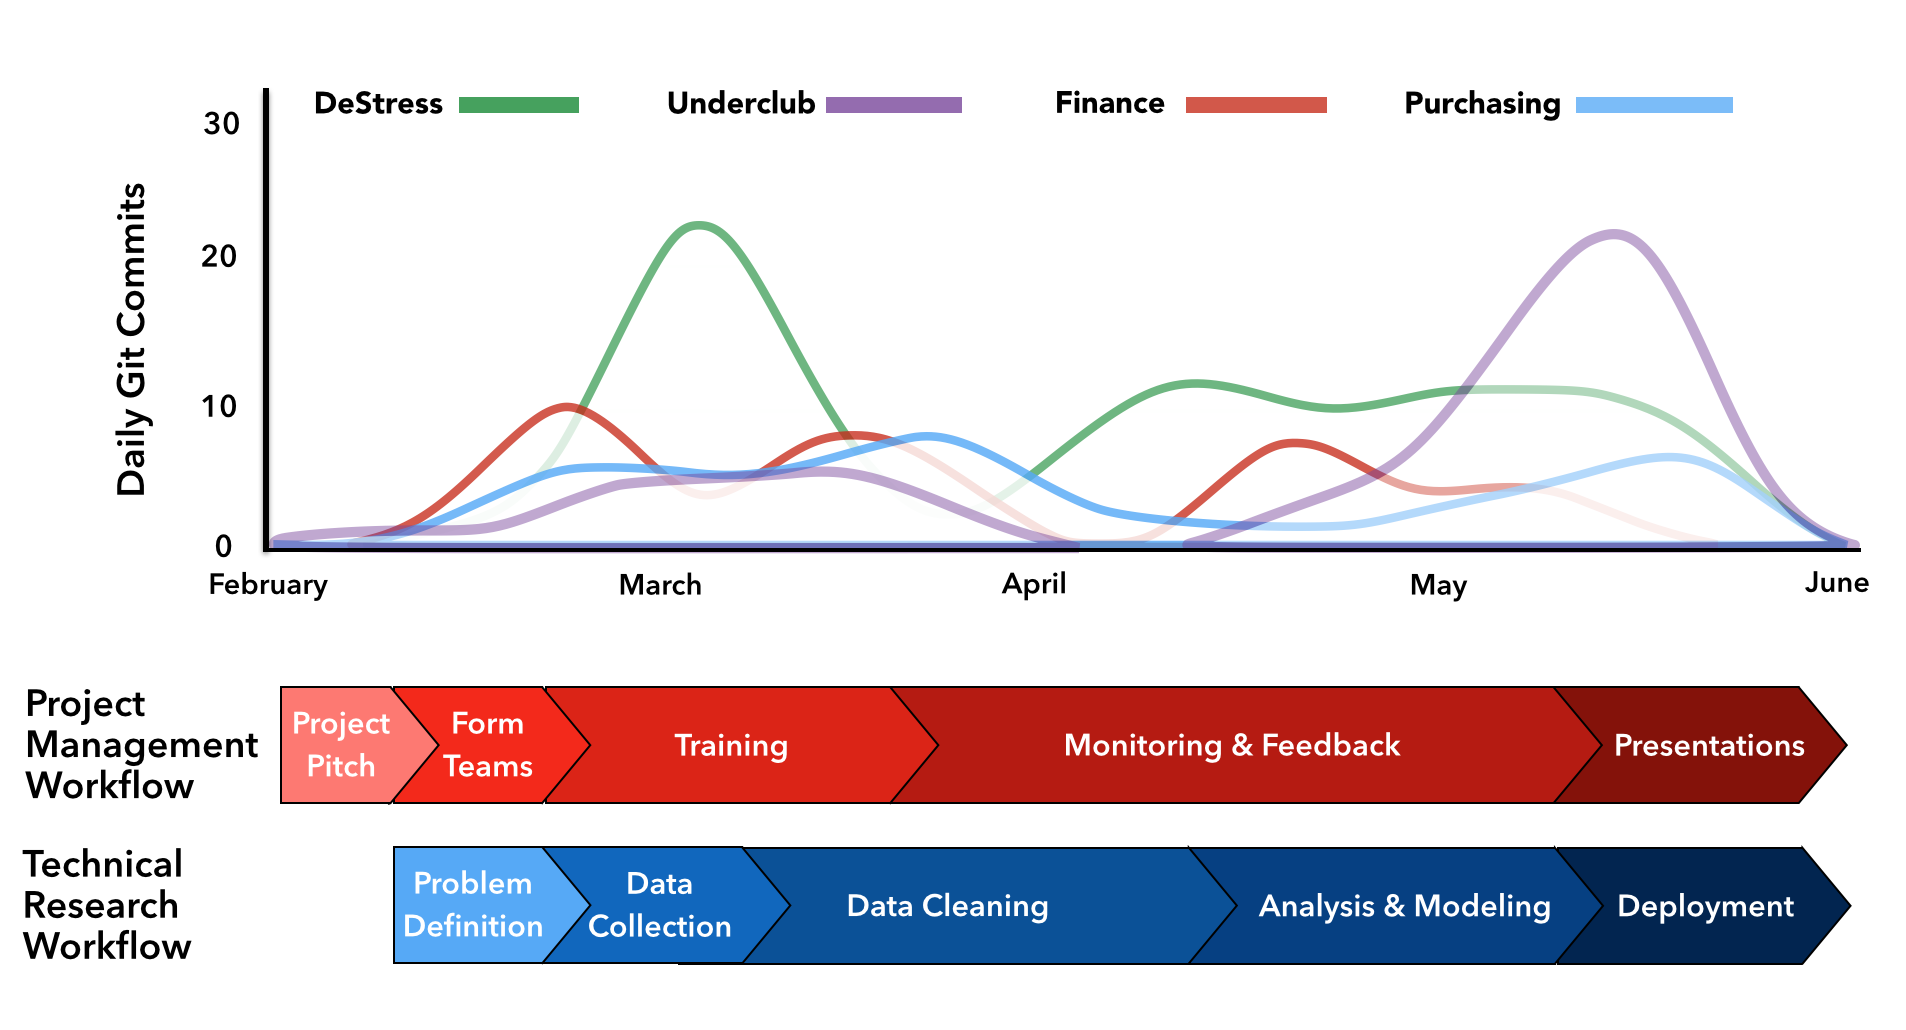
\includegraphics[scale=0.5]{BIDS_Collaborative_Workflow.png}}
\centerline{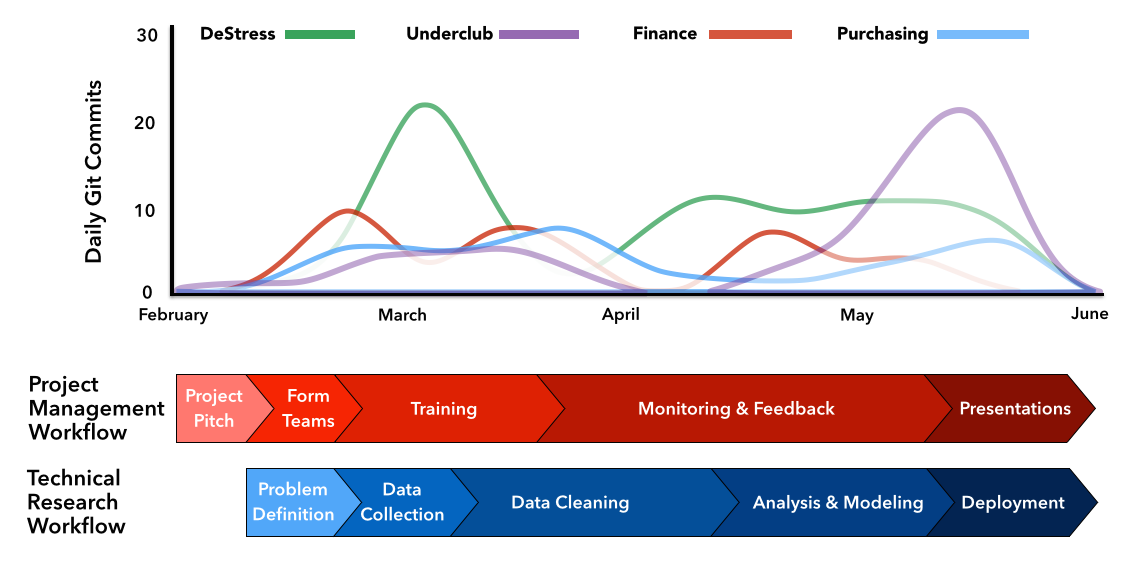
\includegraphics[scale=0.435]{BIDS_Collaborative_Workflow_NEW.png}}
\caption{GitHub commit histories of BIDS Collaborative teams overlaid with project management and technical research workflows.}
\label{fig:gitcommits}
\end{figure*}

The diverse skill levels of the participants further complicated training sessions throughout March. As such the initial period was trying, and again consisted primarily of smaller-scale coaching from facilitators and mentors. The usage of BIDS space was ad hoc, with some members of the BIDS community finding this usage disruptive. This was addressed by identifying a single weekday where Collaborative participants were particularly encouraged to attend and ``take over" the space, and to be particularly conscientious outside of this time.

This DeStress project maintained robust activity throughout the semester, perhaps exemplifying the ideal project workflow.  Team members were especially active during the early training sessions, coinciding with their data collection and data cleaning work.  This placed the team in a strong position for the remainder of the semester, where members were competent in the usage of tools and well-prepared for the analysis and modeling phase.  This project produced excellent technical research and final presentation, and the participants are currently working towards several publications resulting from this work.

Underclub participants struggled in the early stages, and team members lagged in adopting the collaborative tools.  As a result this project produced few actionable insights, as was apparent in their final presentation, although some promising directions were established. It is clear that more guidance was needed to efficiently connect their analyses with potential business-relevant actions.  A further shortcoming of the Underclub project was the failure to create a public repository, which would serve as a public record of team progress. This is somewhat understandable, however, given the relatively short timeframe of a single academic semester.  Some efforts were made at the conclusion of this project to create open version of the work for public consumption, as is indicated by the final team push through the deployment phase.

Unlike other projects, the Finance project incurred non-trivial startup overhead.  This included software installation challenges, and integration with the traditional HPC Scheduler. As such, much of the semester was spent attaining proof-of-concept workflows using Spark to analyze a subset of the full dataset.  Having achieved this proof-of-concept, the Finance project has led to continued work in the D-Lab, though primarily with a different set of contributors. This transition underscores the value of working in public repositories for genuinely open-ended projects, where new contributors can pick up where previous efforts left off.

The Purchasing project demonstrated the difficulties for a team of graduate students to obtain actionable insights from working only a few hours per week for for semester.  Team activity and progress were slow throughout the course of the Collaborative.  Some progress was made, however, in identifying basic workflows and determining which questions appear to be answerable. In particular, clustering techniques showed promise in identifying subtle partnerships, where collective purchasing could provide savings.  As a result of modest efforts, this project produced a minimal set of useful results.



\section{Lessons Learned}

The first iteration of the BIDS Collaborative was an experimental undertaking, in which both participants and Collaborative facilitators were jointly learning throughout.  The Collaborative experienced both successes and failures, and many lessons for effective data science education became apparent.  These lessons have been documented internally, and will serve as guides for subsequent iterations of the Collaborative. These lessons help motivate our final hypothesis addressing the ingredients necessary for effective data science education.

\subsection{Project Vetting}

Using our model where students select among pre-determined projects, it is important to present options representing a broad variety of disciplines.  For example, having projects relating to physical sciences, social sciences, technology, health, environment, commerce, among many other possibilities.  The Collaborative was very successful in this manner.  By presenting this diverse range of project options, we were able to leverage students' innate interests in particular areas of study; thus, students did not feel shoehorned into a research areas of little or no interest to them.

The careful framing and acquisition of data for projects was necessary for project success.  Specifically, the logistics of each project must be fully in order and have a well-defined goal.  Only projects fitting this mold were adopted by students in the Collaborative, while other projects languished.  This extended to having a responsive and dedicated individual representing the underlying client organization.  And most importantly, the relevant data must be available in advance, such that students could get a sense of the project and could begin work immediately.  This consideration of projects also encompasses any legal releases or non-disclosure agreements pertaining to data access.

\subsection{Leadership and Team Formation}

The Collaborative was not entirely successful in organizing the initial process of project team formation.  This led to a difficult first month for everyone involved.  We conclude that project and team components must be organized in the appropriate order.  This should begin by identifying clients with data science research projects of the appropriate scale.  The next step is to identify student team leads who are capable of leading a research team and interacting with the client.  Once this organization in place, it is possible to assemble team members for each project based on students' interests and skill sets.  We conclude that only by following this order of \emph{client, data, team lead, team members}, will each step flow smoothly in succession.

For the upcoming Fall 2015 Collaborative, we will utilize this lesson and initially identify team leads for each project.  At this point, facilitators can work with team leads to select remaining team members. This will serve to simplify and distribute the process of team formation, while also clearly establishing a leadership role for the team lead from the onset of each project.

We observed that regular interaction between each client and team lead was necessary. Team leads served as the bridge for processing and presenting the client needs to team members.  It was not possible for the Collaborative facilitators to fill this role.  It was impractical to micro-manage each project at this level, and requiring this direct interaction between clients and team leads allowed students to self-organize and themselves undertake real-world research projects.  This approach provided a sense of responsibility and accomplishment for team leaders and team members.

\subsection{Milestones}

The Collaborative was successful at creating well-defined intermediate goals, which helped maintain momentum throughout the semester.  These goals took for the form of data-centric ``milestones," such as completing data cleaning, or preliminary data exploration.  Formally assigning dates for these milestones ensured forward progress.  In addition, this helped the Collaborative facilitators passively monitor the progress of individual teams, and provide additional help when necessary.  Larger milestones included a mid-semester presentation, and a capstone evening event including final presentations to the client organizations.  We consider these milestones as being critical to the short-term nature of an academic semester.

\subsection{Training and Tools}

The Collaborative was not entirely successful at the early introduction or promotion of collaborative tools.  The most successful project teams immediately adopted GitHub for all project code, and also Slack for team communications.  It appeared that the sooner team members adopted these tools into their research workflows, the sooner meaningful progress began.  We conclude it is critical to introduce these tools to students early, and promote, if not mandate their usage for teamwork and communications.

In the upcoming iteration of the Collaborative, we have adopted a clear plan for the beginning of the semester. Students will attend a weekly practicum that will include orientations to technical tools, collaborative tools, and project management and documentation.



\section{Closing}

A number of open questions remain from the first iteration of the BIDS Collaborative.  We discuss several of these questions, then present our conclusions and hypothesis for future data science education.

\subsection{Open Questions}

We explored possibilities for offering academic credit as motivation for students, but no students decided to pursue this option. The reason behind this remains uncertain, though it could be due to the lack of structure and the additional hurdles in enrollment. We believe one pathway would be creating a framework that plugs into an existing or a new project-oriented course, an option we are exploring in the Fall.  Even so, however, the option of receiving course credit did not appear to be a strong motivation for students.

Some fraction of students, however motivated, were not prepared with the technical background for jumping into a data science research project.  The usefulness of periodic training sessions, and how these could be organized or delivered, remains an open question.  Who would teach such sessions and exactly what material would be most beneficial for students is also unclear.  This training could possibly overlap with existing workshop or training programs on campus, so certain students have the opportunity to get up to speed on the relevant tools.

The best approach to organizing, managing, and motivating teams remains unclear to the facilitators.  One approach would be to micromanage to some degree, and organize regular weekly team meetings.  However, this level of management is very time-consuming, and not always effective or appreciated by student groups.  Similarly, how to motivate a strong commitment from team members is a difficult question.  Fundamentally, we would like to rely on students' desires for real-world data science experience and education, but this will not always suffice.  How all students can be effectively motivated remains open for discussion.

\subsection{Conclusions}

The BIDS Collaborative was a small educational experiment done in BIDS with a bare bones staff and limited advance planning. We did not have the resources of the DSSG program, but we were successful in motivating a group of students to complete client provided real-world data science problems over the course of an academic semester.  The design and overall success of the BIDS Collaborative program shows promise in terms of scalability at the wider university level.

In addition, the first iteration of the Collaborative brought a variety of practical considerations for effective data science education to light.  Perhaps foremost is the importance of having real-world projects, which represent interested clients and are backed by accessible data, ready at hand.  Forethought about the relationships and communication lines between clients, projects team leads, and team members was also proved surprisingly important for the smooth operation of the research teams.  Finally, the early introduction and training of the appropriate technical tools was also necessary for effective team dynamics.

We hypothesize that effective multidisciplinary data science education must address the complexities which are fundamental to both technical research and human team dynamics. This requires imposing a structured hierarchy for client-team dynamics, augmented with workshops and consulting services to provide the resources necessary for productive research, and most importantly, we note the value of a capstone collaborative project which provides genuinely experiential learning, which we feel is most beneficial for effective data science education.

Stepping back, we have determined best practices from the various approaches applied to creating multidisciplinary teams to solve real life challenges.  Although these lessons arose from a semester-long program for experiential data science education, they can be applied equally well to experiential learning in other disciplines.  We believe our general conclusions may benefit project-based educational programs throughout university systems as a whole.



A huge gaping need for project-based learning.
Challenges faced in industry are different from what is taught in traditional courses.
Needs this model of education.
Pedogodgy which could be used for the future of data science education.
Re-engineer the academic curriculum to make this scalable, without too much overhead of staff for training.
Can do it with clients, minimal staff, and students, in the context of apprenticiship, which is missing from the exisitng educatinal paradigm.
Grand motivation behind it all.
Exisiting research project undertakings are *not* done for the purposes of scalable educational development.
For advancement of educational pedogodgy.
No one else 

DSSG said
Data Kind is not focudes on education.
Bayes Impact is not focussed on education.
The summer program (fellows, etc) is not scalable.
If he could redo it, he wouldn't follow that model.
There needs to be an effort to find out how to make data science, or experiential project-based data science work scalable across a university.
This the attempt to create the social and scientific advancements possible.
There is no model right now for this that's scalaable for data science education, which would have such an impact at the university level.  A way to leverage university resources to provide this new model of project-based education.  


\newpage

%\bibliographystyle{apa}
%\bibliography{ZoteroLibrary}

\newpage
\printbibliography

\end{document}





